\chapter{Marco Teórico \label{cap:teo}}

En este capítulo se desarrollarán las herramientas analítico-teóricas que permiten describir los sistemas fótonicos estudiados en esta tesis. Estos consisten en la propagación de luz láser de baja potencia\footnote{1 mW de potencia de salida, dentro del régimen de seguridad de láseres tipo 3b.} propagada en sistemas acoplados de guías de ondas, las cuales están escritas dentro de una muestra de vidrio de borosilicato. Estas condiciones experimentales permiten describir el comportamiento de la luz utilizando las ecuaciones de Maxwell aplicadas a un medio lineal, isotrópico, no magnético y sin fuentes de carga ni de corriente libres. 
\section{Propagación en guías de ondas dieléctricas desde las ecuaciones de Maxwell \label{cap:maxwell}}

Las ecuaciones de Maxwell en este régimen, en el Sistema Internacional de Unidades, son:
\begin{align}
	\nabla\cdot\left[\varepsilon(\textbf{r})\textbf{E}\right] &= 0 \ , \label{eqn:gauss}
	\\	
	\nabla\times\textbf{E} &= -\mu_0 \frac{\partial \textbf{H}}{\partial t} \ , \label{eqn:faraday-lenz}
	\\	
	\nabla\cdot\textbf{H} &= 0 \ , \label{eqn:div0}
	\\	
	\nabla\times\textbf{H} &=\varepsilon(\textbf{r}) \frac{\partial \textbf{E}}{\partial t} \ , \label{eqn:ampere-maxwell}
\end{align}
donde \textbf{E} es el campo eléctrico y \textbf{H} es el campo magnético. En general, las guías de ondas consideradas son sistemas invariantes en la dirección de propagación $\hat{\textbf{z}}$. Por lo tanto, el perfil de índice de refracción puede expresarse como $n(x,y) = n_0 + \Delta n(x,y)$ donde $n_0 = 1.48$ es el índice de refracción del sustrato de borosilicato y $\Delta n(x,y)$ representa la modulación transversal del índice, con valores máximos en el rango de $10^{-5} - 10^{-3}$. Esta variación espacial del índice, $\Delta n(x,y)$, es responsable del confinamiento óptico en el plano transversal $(x,y)$, permitiendo la propagación guiada de los modos electromagnéticos a lo largo del eje $\hat{\textbf{z}}$. 

Luego de asumir una solución temporal armónica proporcional a $e^{-i\omega t}$ se puede reemplazar la ecuación de Faraday-Lenz (\ref{eqn:faraday-lenz}) en la de Ampère-Maxwell (\ref{eqn:ampere-maxwell}) obteniendo:
\begin{align}
	\nabla\times\left(\frac{\nabla\times\textbf{E}}{i\omega\mu_0}\right) &= -i\omega \varepsilon_0 n^2 \textbf{E} \implies \nabla\times\nabla\times\textbf{E} = k_0^2n^2\textbf{E} \ , \label{eqn:rotordoble}
\end{align}
donde $k_0 \equiv \omega/c$ es el número de onda en el vacío. Por identidad de cálculo vectorial, se tiene que $\nabla\times\nabla\times\textbf{E} = \nabla(\nabla\cdot\textbf{E}) - \nabla^2\textbf{E}$. La ley de Gauss (\ref{eqn:gauss}) implica que $\nabla\cdot \textbf{E} = -\frac{\nabla n^2}{n^2}\cdot\textbf{E}$. Al reemplazar en la ecuación (\ref{eqn:rotordoble}), se obtiene la ecuación 
\begin{equation}
	\left(\nabla^2  + k_0^2n^2\right)\textbf{E} = -\nabla\left( \frac{\nabla n^2}{n^2} \cdot \textbf{E}  \right) \ . \label{eqn:helmholz}
\end{equation}
Análogamente, es posible aplicar combinar las ecuaciones de Ampère-Maxwell (\ref{eqn:ampere-maxwell}) y de Faraday-Lenz (\ref{eqn:faraday-lenz}) en conjunto con la divergencia nula del campo magnético \textbf{H} (\ref{eqn:div0}):
\begin{align}
	\nabla\times \left(\frac{\nabla\times\textbf{H}}{-i\omega \varepsilon_0 n^2}\right) = i\omega \mu_0 \textbf{H} &\implies \nabla\times \left(\frac{1}{n^2}\nabla\times\textbf{H}\right) = k_0^2 \textbf{H} \ ,
	\nonumber
	\\
	\nabla\times\nabla\times\textbf{H} + \nabla n^2 \times \left( \nabla\times\textbf{H}\right)
	&= 
	  k_0^2 n^2\textbf{H} \ .
	 	\nonumber
\end{align}
La ecuación análoga a (\ref{eqn:helmholz}) para \textbf{H} es, por consiguiente:
\begin{align}
	 \left(\nabla^2  + k_0^2 n^2 \right) \textbf{H} &= i\omega \epsilon_0 \nabla n^2 \times \textbf{E} \ .
	 \label{eqn:helmholzH}
\end{align}
En esta tesis se trabajará con sistemas en los que la luz viaja a través de una estructura de guías de ondas constantes en la dirección $\hat{\textbf{z}}$ y periódicas en la dirección transversal. Es por ello que será útil separar los componentes longitudinales y transversales de los campos, asumiendo una dependencia del tipo onda plana $e^{i k_z z}$ en la variable espacial $z$:
\begin{align}
	\nabla_\perp \times  \textbf{E} + ik_z \hat{\textbf{z}} \times \textbf{E} &= i\omega\mu_0\textbf{H} \ ,
	\label{eqn:EfieldH}
	\\
	\nabla_\perp \times  \textbf{H} + ik_z \hat{\textbf{z}} \times \textbf{H} &= -i\omega \epsilon_0 n^2 \textbf{E} \ .
	\label{eqn:HfieldE}
\end{align}
Si se consideran las descomposiciones $\textbf{E}=\textbf{E}_\perp +\hat{\textbf{z}} E_z$ y $\textbf{H}=\textbf{H}_\perp +\hat{\textbf{z}} H_z$, $\nabla_\perp \equiv - \hat{\textbf{z}}\times (\hat{\textbf{z}}\times\nabla)   $, las ecuaciones de Maxwell que involucran rotores se escriben como:
\begin{align}
	\nabla_\perp \times  \textbf{E}_\perp + ik_z \hat{\textbf{z}} \times \textbf{E}_\perp + \nabla_\perp \times (\hat{\textbf{z}} E_z) &= i\omega\mu_0(\textbf{H}_\perp +\hat{\textbf{z}} H_z) \ ,
	\label{eqn:Efield}
	\\
	\nabla_\perp \times  \textbf{H}_\perp + ik_z \hat{\textbf{z}} \times \textbf{H}_\perp + \nabla_\perp \times (\hat{\textbf{z}} H_z) &= -i\omega \epsilon_0 n^2 (\textbf{E}_\perp +\hat{\textbf{z}} E_z) \ .
	\label{eqn:Hfield}
\end{align}
Luego de aplicar producto cruz en la dirección $\hat{\textbf{z}}$ a las ecuaciones (\ref{eqn:Efield}) y (\ref{eqn:Hfield}), se puede expresar $E_z$ y $H_z$ en función de $\textbf{E}_\perp$ y $\textbf{H}_\perp$:
\begin{equation*}
\begin{aligned}[c]
	 -i\nabla_\perp E_z &= k_z\textbf{E}_\perp +\omega \mu_0 \hat{\textbf{z}} \times \textbf{H}_\perp \ ,
	 	  	 \\
	 	  	i\hat{\textbf{z}} \times \nabla_\perp H_z &= k_z \hat{\textbf{z}} \times\textbf{H}_\perp + \omega\epsilon_0 n^2 \textbf{E}_\perp \ ,
\end{aligned} 
\quad
\begin{aligned}[c]
	-i \nabla_\perp H_z &= k_z \textbf{H}_\perp - \omega \epsilon_0 n^2  \hat{\textbf{z}} \times \textbf{E}_\perp \ ,
	\\
	i\hat{\textbf{z}} \times\nabla_\perp E_z &=  \omega \mu_0 \textbf{H}_\perp+k_z  \hat{\textbf{z}} \times \textbf{E}_\perp \ .
\end{aligned}
\end{equation*}
Finalmente, los componentes perpendiculares de los campos, $\textbf{H}_\perp$ y $\textbf{E}_\perp$, se pueden despejar en términos de los componentes longitudinales, $H_z$ y $E_z$:
\begin{equation}
\begin{aligned}[c]
 \hat{\textbf{z}} \times \textbf{H}_\perp &= i\frac{(\omega\epsilon_0 n^2 \nabla_\perp E_z  - \hat{\textbf{z}} \times \nabla_\perp H_z k_z)}{k_0^2 n^2 - k_z^2} \ ,
 \\
\textbf{H}_\perp &= \frac{i}{k_0^2 n^2 - k_z^2}\left(k_z\nabla_\perp H_z + \omega \epsilon_0 n^2\hat{\textbf{z}} \times \nabla_\perp E_z\right) \ ,
\end{aligned}
\begin{aligned}[c]
	\hat{\textbf{z}} \times \textbf{E}_\perp &= -i\frac{(k_z\hat{\textbf{z}} \times \nabla_\perp E_z + \omega\mu_0 \nabla_\perp H_z)  }{k_0^2 n^2 - k_z^2} \ ,
	\\
\textbf{E}_\perp &= \frac{i}{k_0^2 n^2 - k_z^2}\left(k_z \nabla_\perp E_z - \omega\mu_0 \hat{\textbf{z}} \times \nabla_\perp H_z\right) \ . \label{eqn:transversal}
\end{aligned}
\end{equation}
Las ecuaciones (\ref{eqn:helmholz}), (\ref{eqn:helmholzH}) y (\ref{eqn:transversal}) serán las herramientas analíticas para los dos casos de estudio de las siguientes secciones.
\section{Soluciones analíticas para guías de ondas tipo placa o \textit{slab} unidimensionales \label{cap:slab}}
El sistema más simple que se puede estudiar es una guía de ondas tipo placa, cuya forma analítica para el contraste $n(x)$ es la siguiente:
\begin{equation*}
	n(x) = \left\{\begin{matrix}
	n_1 \ , \quad |x| \le a
	\\
	n_0 \ , \quad |x| > a
 	\end{matrix}\right. \ ,
\end{equation*}
con $n_1 > n_0$. \begin{figure}[H]
	\centering
	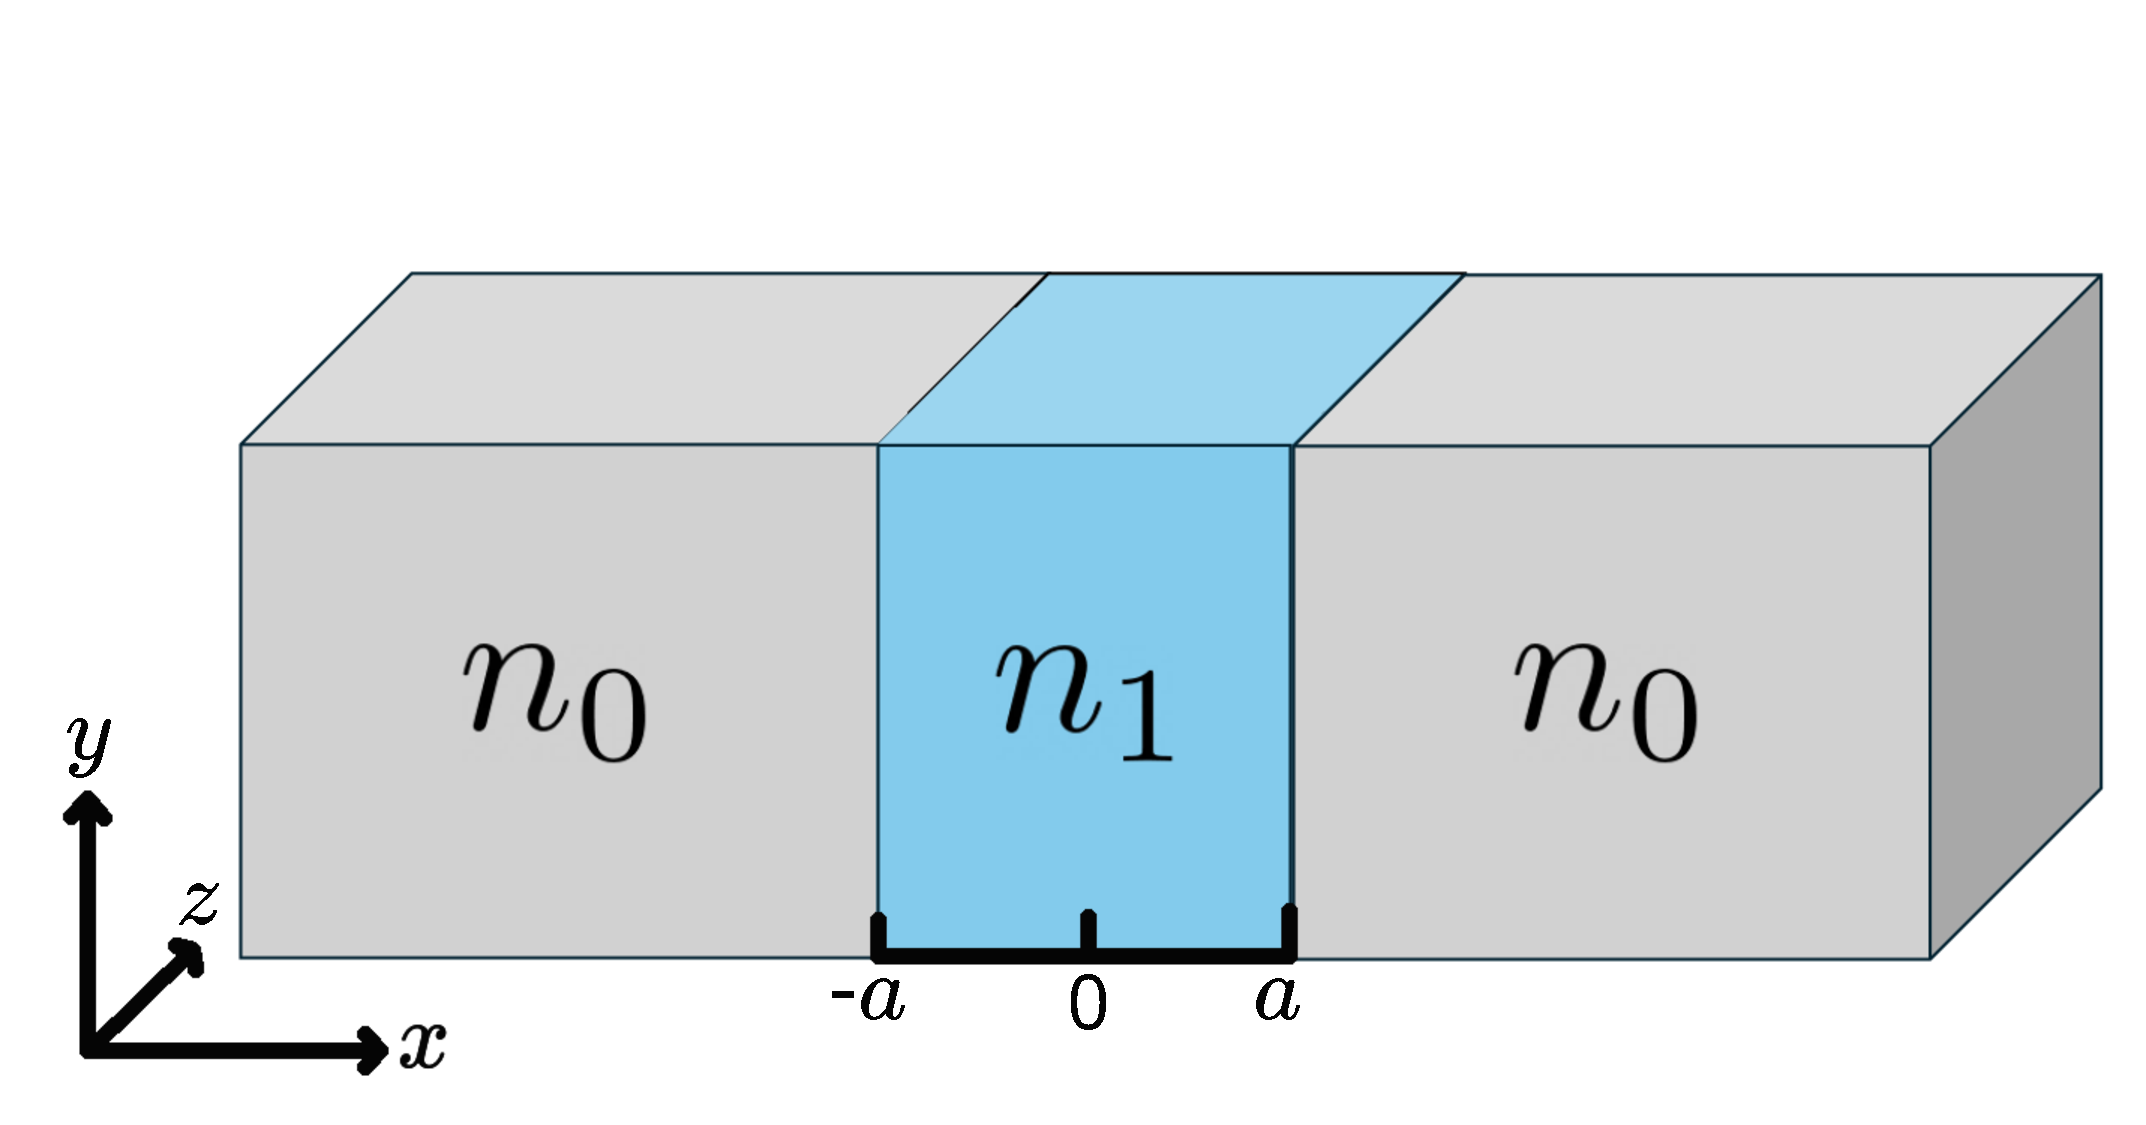
\includegraphics[width=0.6\linewidth]{media/slab.pdf}
	\caption[Forma de una guía de ondas tipo placa.]{Forma de una guía de ondas tipo placa. En las direcciones $\mathbf{\hat{y}}$ (vertical) y $\mathbf{\hat{z}}$ (hacia dentro de la página) la estructura es invariante.}
\end{figure} Dado que $\nabla n^2 = \textbf{0}$ para $|x| \neq a$, los lados derechos de las ecuaciones (\ref{eqn:helmholz}) y (\ref{eqn:helmholzH}) son de tipo Helmholtz. Definiendo $\Psi = \{E_z, H_z\} $:
\begin{align*}
	(\nabla_\perp^2  + k_0^2n^2 - k_z^2) \Psi  &=  \frac{d^2\Psi}{dx^2} + (k_0^2n^2 - k_z^2) \Psi  = 0 \ .
\end{align*}
Como $n(x)=n(-x)$, las soluciones $\Psi$ deben ser pares o impares. En efecto, si $\Psi(x)$ es solución, el cambio $x\to x'=-x$ implica que $\Psi(-x)=\pm \Psi(x)$, pues $\Psi(x)$ es un campo real.
Para encontrar soluciones cuya energía esté localizada en la guía de ondas y que decaiga fuera de ella, se impondrá $k_0^2n_0^2 \le k_z^2 \le k_0^2n_1^2$. Se hace natural definir $\alpha^2\equiv k_0^2n_1^2-k_z^2$ y $\beta^2\equiv k_z^2 - k_0^2n_0^2$. Con todo esto, 
\begin{equation*}
	\Psi_s = \left\{\begin{matrix}
	\Psi_{s1}\cos(\alpha x) \ , & |x|\le a
	\\
	\Psi_{s0}e^{-\beta|x|} \ , & |x|>a
	\end{matrix}\right.
	\
	\implies 	
	\	
	\nabla_\perp \Psi_s = \left\{\begin{matrix}
	-\hat{\textbf{x}}\alpha\Psi_{s1}\sin(\alpha x) \ , & |x|\le a
	\\
	-\hat{\textbf{x}}\frac{|x|}{x}\beta\Psi_{s0}e^{-\beta|x|} \ , & |x|>a
	\end{matrix}\right.
	\
	.
\end{equation*}
Por lo que las componentes verticales $E_y$ y $H_y$ pares se escriben debido a la ecuación (\ref{eqn:transversal}) como:
\begin{equation*}
	\begin{aligned}[c]
	 E_y &= \frac{i \omega\mu_0}{k_0^2n^2-k_z^2} \left\{\begin{matrix}
	 \alpha H_{s1}\sin(\alpha x) \ ,	 & |x|\le a
	 \\
	 \frac{|x|}{x}\beta H_{s0}e^{-\beta|x|} \ , & |x|>a
	 \end{matrix}\right.
\end{aligned} 
,\quad
	\begin{aligned}[c]
	 H_y &= \frac{-i\omega \epsilon_0 n^2}{k_0^2n^2-k_z^2} \left\{\begin{matrix}
	 \alpha E_{s1}\sin(\alpha x) \ ,	& |x|\le a
	 \\
	 \frac{|x|}{x}\beta E_{s0}e^{-\beta|x|} \ , & |x|>a
	 \end{matrix}\right.
	 \
	 .
\end{aligned} 
\end{equation*}
Por otro lado, las soluciones impares tienen la forma
\begin{equation*}
	\Psi_a = \left\{\begin{matrix}
	\Psi_{a1}\sin(\alpha x) \ , & |x|\le a
	\\
	\Psi_{a0}e^{-\beta|x|} \ , & |x|>a
	\end{matrix}\right.
	\
	\implies
	\
		\nabla_\perp \Psi_a = \left\{\begin{matrix}
	\hat{\textbf{x}}\alpha\Psi_{a1}\cos(\alpha x) \ , & |x|\le a
	\\
	-\hat{\textbf{x}}\frac{|x|}{x}\beta\Psi_{a0}e^{-\beta|x|} \ , & |x|>a
	\end{matrix}\right.
	\
	.
\end{equation*}
Por lo que $E_y$ y $H_y$ se escriben como:
\begin{equation*}
	\begin{aligned}[c]
	 E_y &= \frac{i\omega\mu_0}{k_0^2n^2-k_z^2} \left\{\begin{matrix}
	 -\alpha H_{a1}\cos(\alpha x) \ , & |x|\le a
	 \\
	 \frac{|x|}{x}\beta H_{a0}e^{-\beta|x|} \ , & |x|>a
	 \end{matrix}\right.
\end{aligned} 
,\quad
	\begin{aligned}[c]
	 H_y &= \frac{i\omega \epsilon_0 n^2}{k_0^2n^2-k_z^2} \left\{\begin{matrix}
	  \alpha E_{a1}\cos(\alpha x) \ ,	 & |x|\le a
	 \\
	 -\frac{|x|}{x}\beta E_{a0}e^{-\beta|x|} \ , & |x|>a
	 \end{matrix}\right.
\end{aligned} .
\end{equation*}
Imponiendo continuidad de las componentes tangenciales $E_y$, $E_z$, $H_y$ y $H_z$:
\begin{equation*}
	\begin{aligned}[c]
	 E_{s1}\cos(\alpha a) = E_{s0}e^{-\beta a} \ ,
	 \\	 
	 H_{s1}\cos(\alpha a) = H_{s0}e^{-\beta a} \ ,
	 \\
	 	  n_1 ^2 E_{s1}\sin(\alpha a)/\alpha = -n_0^2 E_{s0}e^{-\beta a}/\beta \ ,
	  \\
	  H_{s1}\sin(\alpha a)/\alpha = - H_{s0}e^{-\beta a}/\beta \ ,
\end{aligned} 
\quad
	\begin{aligned}[c]
		 E_{a1}\sin(\alpha a) = E_{a0}e^{-\beta a} \ ,
	 	   \\
	 H_{a1}\sin(\alpha a) = H_{a0}e^{-\beta a} \ ,
	 \\
	  n_1 ^2 E_{a1}\cos(\alpha a)/\alpha = n_0^2 E_{a0}e^{-\beta a}/\beta \ ,
	 	 \\
	  H_{a1}\cos(\alpha a)/\alpha = H_{a0}e^{-\beta a}/\beta \ .
\end{aligned} 
\end{equation*}
Buscando soluciones no triviales se tiene que:
\begin{equation*}
	\left[\frac{\cos(\alpha a)}{\beta a} + \frac{\sin(\alpha a)}{\alpha a}\right] \left[n_0^2 \frac{\cos(\alpha a)}{\beta a} + n_1^2\frac{\sin(\alpha a)}{\alpha a} \right]
	 \left[ \frac{\sin(\alpha a)}{\beta a} - \frac{\cos(\alpha a)}{\alpha a}\right]\left[ n_0^2\frac{\sin(\alpha a)}{\beta a} - n_1^2\frac{\cos(\alpha a)}{\alpha a}\right] = 0
\end{equation*}
Se distinguirá dos tipos de condiciones:
\begin{itemize}
	\item Modos eléctricos transversales (TE):\begin{align}
	\frac{\cos(\alpha a)}{\beta a} + \frac{\sin(\alpha a)}{\alpha a}&= 0 \ , \label{eqn:TEsim}
	\\
	 \frac{\sin(\alpha a)}{\beta a} - \frac{\cos(\alpha a)}{\alpha a} &= 0 \ . \label{eqn:TEanti}
	\end{align}
	\item Modos magnéticos transversales (TM):\begin{align}
	n_0^2 \frac{\cos(\alpha a)}{\beta a} + n_1^2\frac{\sin(\alpha a)}{\alpha a}  &= 0 \ , \label{eqn:TMsim}
	\\
	 n_0^2\frac{\sin(\alpha a)}{\beta a} - n_1^2\frac{\cos(\alpha a)}{\alpha a} &= 0 \ . \label{eqn:TManti}
	\end{align}
\end{itemize}
Asumiendo $\alpha$, $\beta$ y $k_z$ conocidos, las amplitudes deben cumplir las relaciones:
\begin{equation*}
	\begin{aligned}[c]
	E_{s1} \left[n_0^2 \frac{\cos(\alpha a)}{\beta a}+n_1 ^2 \frac{\sin(\alpha a)}{\alpha a}\right] = 0 \ ,
		\\
	H_{s1} \left[\frac{\cos(\alpha a)}{\beta a} + \frac{\sin(\alpha a)}{\alpha a} \right] = 0 \ ,
\end{aligned} 
\quad\quad
	\begin{aligned}[c]
	E_{a1} \left[ n_0^2\frac{\sin(\alpha a)}{\beta a} - n_1^2\frac{\cos(\alpha a)}{\alpha a}\right] = 0 \ ,
		\\
	H_{a1} \left[ \frac{\sin(\alpha a)}{\beta a} - \frac{\cos(\alpha a)}{\alpha a}\right] = 0 \ .
\end{aligned} 
\end{equation*}
Las ecuaciones superiores imponen que $E_1 = 0$ cuando se satisface alguna condición de modos TE. Análogamente, las ecuaciones inferiores imponen $H_1 = 0$ en el caso de modos TM, lo que impone transversalidad en la oscilación de los campos respectivos.
Un corolario para los modos TE es que $E_z = E_x = 0$, por lo que la polarización del campo eléctrico será exclusivamente en la dirección $\hat{\textbf{y}}$. Así mismo, sólo un haz polarizado en $\hat{\textbf{x}}$ podría excitar un modo TM, por lo que en un experimento se debe tener esto presente: una condición inicial arbitraria se propagará como una combinación lineal de los modos TE y TM que soporte la guía.

\subsection{Soluciones gráficas y comparación entre modos TE y TM \label{cap:solslabTETM}}

Usando las dos ecuaciones de modos TE junto a la restricción $(\alpha a)^2 + (\beta a)^2 = k_0^2 a^2(n_1^2 - n_0^2) \equiv V^2$ es posible obtener soluciones gráficas para las constantes de propagación $k_z$ a partir de las intersecciones $(\alpha a, \beta a)$, como se grafica en la Figura \ref{fig:graphTE}. La cantidad de modos aumenta con la diferencia entre índices de refracción.

\begin{figure}[H]
	\centering
	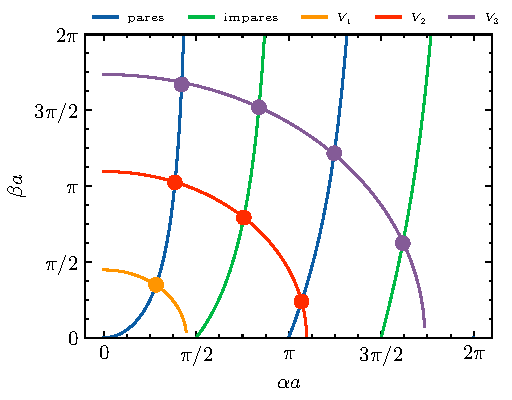
\includegraphics[width=0.5\linewidth]{media/slabgraphical.pdf}
	\caption[Soluciones gráficas de los modos TE.]{Soluciones gráficas de los modos TE. A mayor contraste $\Delta n = n_1-n_0$, mayor cantidad de modos guiados soporta la guía de ondas. \label{fig:graphTE}}
\end{figure}
Luego de encontrar $k_z$, se tiene todo lo necesario para reemplazar en las expresiones obtenidas para las componentes del campo electromagnético. En la Figura \ref{fig:E-slab-graph} se grafica la forma espacial de cuatro modos, que se corresponden con los cuatro puntos morados de la Figura \ref{fig:graphTE}.
\begin{figure}[H]
	\centering
	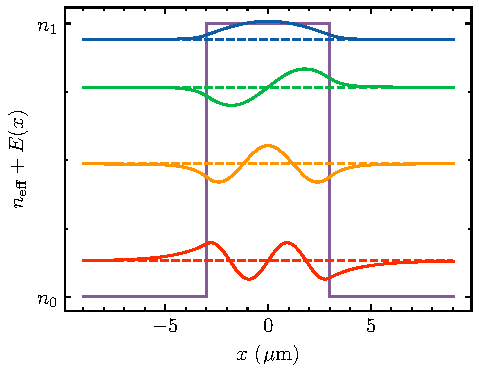
\includegraphics[width=0.5\linewidth]{media/TETMfields.pdf}
	\caption[Forma espacial de la componente longitudinal del campo magnético.]{ Forma espacial de la componente longitudinal del campo magnético. \label{fig:E-slab-graph}}
\end{figure}

La condición de corte (\textit{cutoff}) en guías de ondas es equivalente a que la energía deje de decaer en la región $|x| > a$, es decir, se debe cumplir que $\beta a \to 0$. 
Los modos simétricos o pares cumplen esta condición para $\sin(V) = 0$, lo que implica que $V = m \pi$, con $m$ entero. En particular, considerando $m=0$  y barriendo $n_1 \to n_0$, siempre existen al menos dos modos, uno TE y otro TM mientras $n_1 > n_0$.  
Los modos antisimétricos o impares deben cumplir por su parte que $\cos(V) = 0$, lo que implica que $V = (m\pi \pm \pi/2)$. De esta condición se deduce que el primer par de modos excitados ($m=0$) existe siempre que $\lambda \le \lambda_c \equiv 4a\sqrt{n_1^2-n_0^2}$. Escrito de forma compacta para el $m$-ésimo modo:
\begin{align*}
	 (\lambda_c)_m = \frac{4a}{m-1}  \sqrt{n_1^2-n_0^2} \ ,
\end{align*}
lo que para $a=4 \text{ }\mu$m y $\Delta n = 5\times 10^{-4}$  significa una longitud de onda de corte para el segundo modo de $\lambda_c \approx 615 \text{ nm}$.
\section{Soluciones analíticas para fibra óptica circular}
En la sección anterior se estudió el sistema más sencillo en el que se puede hablar de guías de ondas dieléctricas. El siguiente paso en complejidad consiste en guías de ondas circulares. Para ello, se considerará que el índice de refracción varía radialmente según 
\begin{equation}
	n( \rho ) = 
	\left\{\begin{matrix}
	n_1, \quad \text{si } \rho \le a
	\\
	n_0, \quad \text{si } \rho > a
	\end{matrix}\right.
	\ ,\nonumber
\end{equation}
donde la tupla $(\rho, \phi, z)$ define las coordenadas cilíndricas más apropiadas a usar para este problema. 
Al considerar las componentes longitudinales $\Psi$ = $\{E_z, H_z\}$ del campo eléctrico y magnético y  si se utiliza el método de separación de variables con $\Psi =  R(\rho)\Phi(\phi) e^{ik_z z} $,  las ecuaciones (\ref{eqn:helmholz}) y (\ref{eqn:helmholzH}) toman la forma:
\begin{align}
	\left[\frac{\partial^2}{\partial \rho^2} + \frac{\partial}{\rho\partial \rho} + \frac{\partial^2}{\rho^2\partial \phi^2} +\left( k_0^2n^2 - k_z^2 \right)\right]  R(\rho)\Phi(\phi) = 0
	\nonumber
	\\
\rho^2\frac{d^2 R}{Rd\rho^2} + \rho\frac{dR}{Rd\rho} + \rho^2\left( k_0^2n^2 - k_z^2 \right) + \underbrace{\frac{d^2 \Phi}{\Phi d\phi^2}}_{-\ell^2} = 0
\nonumber
\end{align}
\vspace{-3em}
\begin{align}
\therefore \Phi(\phi) = A e^{i\ell\phi}
\nonumber
\end{align}
Luego de imponer condiciones de periodicidad $\Phi(\phi)=\Phi(\phi + 2\pi)$, se tiene necesariamente que $\ell$ es un número entero. Por consiguiente, la ecuación para $R(\rho)$ es de tipo Bessel entera, por lo que buscando soluciones tales que $k_0^2 n_0^2 < \beta_z^2 < k_0^2 n_1^2$ y definiendo nuevamente $\alpha^2 \equiv k_0^2n_1^2 - k_z^2$ y $\beta^2\equiv k_z^2 - k_0^2n_0^2$ se tiene:
\begin{align}
	\frac{d^2 R}{d\rho^2} + \frac{1}{\rho}\frac{dR}{d\rho} + \left( k_0^2n^2 - k_z^2 -\frac{\ell^2}{\rho^2}\right)R  = 0
	\nonumber
	\\
	\therefore R(\rho) = 
	\left\{
	\begin{matrix}	
	C_1 J_\ell (\alpha\rho) + D_1 Y_\ell (\alpha\rho), \quad \text{si } \rho \le a  
	\\
	C_2 K_\ell (\beta\rho) + D_2 I_\ell (\beta\rho), \quad \text{si } \rho > a  
	\end{matrix}
	\right.
	\ . \nonumber
\end{align}
Necesariamente se debe imponer $D_1 = D_2 = 0$ para que la solución sea finita para $\rho = 0$ y para $\rho \to +\infty$. Es decir, la parte radial de la solución es
\begin{align*}
 R(\rho) = 
	\left\{
	\begin{matrix}	
	C_1 J_\ell (\alpha\rho), \quad \text{si } \rho \le a  
	\\
	C_2 K_\ell (\beta\rho), \quad \text{si } \rho > a  
	\end{matrix}
	\right.
	\ . \nonumber
\end{align*}
En este caso, para imponer las condiciones de continuidad en $\textbf{E}_{||} = E_\phi \boldsymbol{\hat{\phi}} + E_z \hat{\textbf{z}}$ y $\textbf{H}_{||}= H_\phi \hat{\boldsymbol{\phi}} + H_z \hat{\textbf{z}}$, se hace necesario relacionar el resto de componentes del campo con $E_z$ y $H_z$ para lo cual se requieren las ecuaciones (\ref{eqn:transversal}). 

Como 
\begin{equation*}
	\nabla_\perp \Psi =
	\left\{	
	\begin{matrix}
		\Psi_0^1\left[\boldsymbol{\hat{\rho}}\alpha J'_\ell (\alpha \rho) + i \boldsymbol{\hat{\phi}} \ell J_\ell (\alpha \rho)/\rho\right] e^{i\ell\phi} e^{i k_z z} \ , \quad \text{si } \rho \le a  
		\\
		\Psi_0^0\left[\boldsymbol{\hat{\rho}}\beta K'_\ell (\beta\rho) +i \boldsymbol{\hat{\phi}}\ell K_\ell (\alpha \rho)/\rho \right]e^{i\ell\phi} e^{i k_z z} \ , \quad \text{si } \rho > a  
	\end{matrix}
	\right.
\end{equation*}

Separando por componentes y reemplazando:
\begin{align*}
		H_z &=  e^{i\ell\phi}e^{i k_z z}
	  	 \left\{
		\begin{matrix}	  	 
	  	 H_0^1 J_\ell (\alpha \rho) \ , \quad \text{si } \rho \le a  
	  	 \\
	  	 H_0^0 K_\ell (\beta \rho) \ , \quad \text{si } \rho > a  
	  	 \end{matrix}
	  	 \right.	
		\\
	  	 H_r &= \frac{i e^{i\ell\phi}e^{i k_z z} }{k_0^2 n^2 - k_z^2}
	  	 \left\{
		\begin{matrix}	  	 
	  	  k_z \alpha H_0^1 J'_\ell (\alpha \rho) - i\omega \epsilon_0 n^2\ell E_0^1 J_\ell (\alpha \rho)/\rho \ , \quad \text{si } \rho \le a  
	  	 \\
	  	 k_z \beta H_0^0  K'_\ell (\beta \rho) - i\omega \epsilon_0 n^2\ell E_0^0 K_\ell (\beta \rho)/\rho \ , \quad \text{si } \rho > a  
	  	 \end{matrix}
	  	 \right.
	  	 \\
		H_\phi &= \frac{ie^{i\ell\phi} e^{i k_z z}}{k_0^2 n^2 - k_z^2}
		\left\{
		\begin{matrix}
			ik_z\ell H_0^1  J_\ell (\alpha \rho)/\rho + \omega \epsilon_0 n^2  \alpha E_0^1 J'_\ell (\alpha \rho) \ , \quad \text{si } \rho \le a  
			\\
			ik_z \ell H_0^0  K_\ell (\beta \rho)/\rho + \omega \epsilon_0 n^2 \beta E_0^0  K'_\ell (\beta \rho) \ , \quad \text{si } \rho > a  
		\end{matrix}
		\right.
		\\
		E_z &= e^{i\ell\phi} e^{i k_z z}
	  	 \left\{
		\begin{matrix}	  	 
	  	 E_0^1 J_\ell (\alpha \rho) \ , \quad \text{si } \rho \le a  
	  	 \\
	  	 E_0^0 K_\ell (\beta \rho) \ , \quad \text{si } \rho > a  
	  	 \end{matrix}
	  	 \right.	
		\\
	E_r &= \frac{i e^{i\ell\phi} e^{i k_z z} }{k_0^2 n^2 - k_z^2}
	  	 \left\{
		\begin{matrix}	  	 
	  	  k_z \alpha E_0^1 J'_\ell (\alpha \rho)+i\omega \mu_0 \ell H_0^1 J_\ell (\alpha \rho)/\rho \ , \quad \text{si } \rho \le a  
	  	 \\
	  	 k_z \beta E_0^0  K'_\ell (\beta \rho) +i\omega \mu_0 \ell H_0^0 K_\ell (\beta \rho)/\rho \ , \quad \text{si } \rho > a  
	  	 \end{matrix}
	  	 \right.
	\\
	E_\phi &= \frac{i e^{i\ell\phi} e^{i k_z z}}{k_0^2 n^2 - k_z^2}
		\left\{
		\begin{matrix}
			ik_z \ell E_0^1   J_\ell (\alpha \rho)/\rho -\omega \mu_0  \alpha H_0^1  J'_\ell (\alpha \rho) \ , \quad \text{si } \rho \le a  
			\\
			ik_z \ell E_0^0   K_\ell (\beta \rho)/\rho -\omega \mu_0 \beta H_0^0   K'_\ell (\beta \rho) \ , \quad \text{si } \rho > a  
		\end{matrix}
		\right.
\end{align*}
Luego, imponiendo continuidad en $z$ y $\phi$:
\begin{align}
	H_0^{1} J_\ell(\alpha a) &= H_0^{0} K_\ell (\beta a)
	\label{eqn:cont1}
	\\
	E_0^{1} J_\ell(\alpha a) &= E_0^{0} K_\ell (\beta a)
	\label{eqn:cont2}
	 \\
	 -\omega \epsilon_0 n_1^2  \alpha\beta^2 a E_0^1 J'_\ell (\alpha a)-ik_z\ell \beta^2 H_0^1  J_\ell (\alpha a)
	 &= \omega \epsilon_0 n_0^2 \alpha^2 \beta a E_0^0 K'_\ell (\beta a)+ik_z\ell \alpha^2H_0^0  K_\ell (\beta a)
	 \label{eqn:cont3}
	 \\
	 -ik_z \ell \beta^2 E_0^1   J_\ell (\alpha a) + \omega \mu_0  \alpha \beta^2 a H_0^1  J'_\ell (\alpha a) &=
	 ik_z \ell \alpha^2 E_0^0   K_\ell (\beta a) -\omega \mu_0  \alpha^2 \beta a H_0^0  K'_\ell (\beta a)
	 \label{eqn:cont4}
\end{align}
Buscando soluciones no triviales:
\begin{align*}
	\left|\begin{matrix}
		K_\ell(\beta a) & -J_\ell(\alpha a) & 0 & 0
		\\
		0 & 0 & K_\ell(\beta a) & -J_\ell(\alpha a)
		\\
		ik_z\ell \alpha^2 K_\ell (\beta a) & ik_z\ell\beta^2 J_\ell (\alpha a) & \omega \epsilon_0 n_0^2  \alpha^2 \beta a K'_\ell (\beta a) & \omega \epsilon_0 n_1^2  \alpha \beta^2 a J'_\ell (\alpha a)
		\\
		\omega \mu_0  \alpha^2 \beta a   K'_\ell (\beta a) &  \omega \mu_0  \alpha \beta^2 a J'_\ell (\alpha a) & -ik_z \ell \alpha^2 K_\ell (\beta a) &  -ik_z \ell \beta^2  J_\ell (\alpha a)
	\end{matrix}\right|
	=
0
\end{align*}
Finalmente, la ecuación trascendental que satifacen $\alpha$, $\beta$ y $k_z$ es:
\begin{equation}
	\left( \frac{J_\ell'(\alpha a)}{\alpha a J_\ell(\alpha a)} + \frac{K_\ell'(\beta a)}{\beta a K_\ell(\beta a)} \right)\left( n_1^2\frac{J_\ell'(\alpha a)}{\alpha a J_\ell(\alpha a)} + n_0^2\frac{K_\ell'(\beta a)}{\beta a K_\ell(\beta a)} \right) = \ell^2 \left[ \left(\frac{1}{\alpha a}\right)^2 + \left(\frac{1}{\beta a}\right)^2 \right]^2 \left( \frac{k_z}{k_0} \right)^2 . \label{eqn:fiber_trascendental}
\end{equation}
Dado que, en principio, los valores de $k_z$ ya están determinados por la ecuación anterior, es posible obtener dos relaciones entre $H_0^1$ y $E_0^1$:
\begin{align}
\frac{E_0^1}{H_0^1} &=  -\frac{i k_z \ell}{\omega\epsilon_0}\left[ \left(\frac{1}{\alpha a}\right)^2 + \left(\frac{1}{\beta a}\right)^2 \right]  \left[ n_1^2 \frac{J'_\ell(\alpha a)}{\alpha a J_\ell(\alpha a)} + n_0^2 \frac{K'_\ell(\beta a)}{\beta a K_\ell(\beta a)} \right]^{-1} \label{eqn:fiber_polarization_E},
\\
\frac{H_0^1}{E_0^1} &=  \frac{i k_z \ell}{ \omega\mu_0}\left[ \left(\frac{1}{\alpha a}\right)^2 + \left(\frac{1}{\beta a}\right)^2 \right]  \left[ \frac{J'_\ell(\alpha a)}{\alpha a J_\ell(\alpha a)} + \frac{K'_\ell(\beta a)}{\beta a K_\ell(\beta a)} \right]^{-1} \label{eqn:fiber_polarization_H}.
\end{align}
Tomando raíz cuadrada al cociente de las ecuaciones (\ref{eqn:fiber_polarization_E}) y (\ref{eqn:fiber_polarization_H}) se tiene:
\begin{equation}
	\frac{E_0^1}{H_0^1} = i \sqrt{\frac{\mu_0}{\epsilon_0}} \frac{\sqrt{ \frac{J'_\ell(\alpha a)}{\alpha a J_\ell(\alpha a)} + \frac{K'_\ell(\beta a)}{\beta a K_\ell(\beta a)}}}{\sqrt{n_1^2 \frac{J'_\ell(\alpha a)}{\alpha a J_\ell(\alpha a)} + n_0^2 \frac{K'_\ell(\beta a)}{\beta a K_\ell(\beta a)}}} \ .
	\label{eqn:fiber_polarization_simplified}
\end{equation}
\subsection{Modos TE y TM}
El caso más sencillo de estudiar es imponiendo $\ell = 0$. La ecuación (\ref{eqn:fiber_trascendental}) implica:
\begin{align*}
	\frac{J'_{0}(\alpha a)}{\alpha a J_0(\alpha a)} + \frac{K'_0(\beta a)}{\beta a K_0(\beta a)}&=  0 \ , \quad \text{(modos TE)}
	\\
	n_1^2\frac{J'_{0}(\alpha a)}{\alpha a J_0(\alpha a)} + n_0^2 \frac{K'_0(\beta a)}{\beta a K_0(\beta a)} &= 0 \ , \quad \text{(modos TM)}
\end{align*}
De la ecuación (\ref{eqn:fiber_polarization_simplified}) es directo notar que la condiciones de modos transversales que las componentes longitudinales se hacen cero en los casos respectivos: $H_0^1 = 0$ para TE y $E_0^1 = 0$ para TM.

Las condiciones de corte se dan cuando $\beta a \to 0$. Utilizando las expresiones asintóticas para las funciones de Bessel con argumentos pequeños y sus relaciones de recurrencia, se tiene
\begin{align*}
	\frac{\alpha a J_0(\alpha a)}{J_1(\alpha a)}  = -\frac{\beta a K_{0}(\beta a)} {K_1(\beta a)} \approx (\beta a)^2\ln\left(\frac{\beta a e^\gamma}{2}\right) \to 0 \ ,
\end{align*}
por lo que se hace necesario que $\left. J_0(\alpha a)\right|_{\alpha a \to V} = 0$. Denotando $x_{0,m}=$ 2.405,  5.520,  8.654, $\cdots$ al $m$-ésimo cero de la funcion $J_0(x)$, la longitud de onda de corte está dada por 
\begin{equation}
(\lambda_c)_{0,m} = 2\pi a \frac{\sqrt{n_1^2 - n_0^2}}{x_{0,m}} \ , \quad\text{(modos TE y TM)},
\end{equation} 
lo que se traduce en una longitud de onda de corte de $\lambda_c\approx 616$ nm para los mismos parámetros de la sección \ref{cap:slab}, $a=4 \text{ }\mu$m y $\Delta n = 5\times 10^{-4}$ . Contrario al caso de la guía de ondas tipo placa, en fibras ópticas se hace necesario estar bajo un umbral de corte máximo $(\lambda_c)_{0,1}$ no nulo para que los modos TE o TM existan. Como se verá más adelante, esto se debe a que los modos puramente transversales corresponden a modos excitados: el modo fundamental es híbrido.

%\begin{figure}[H]
%	\centering
%	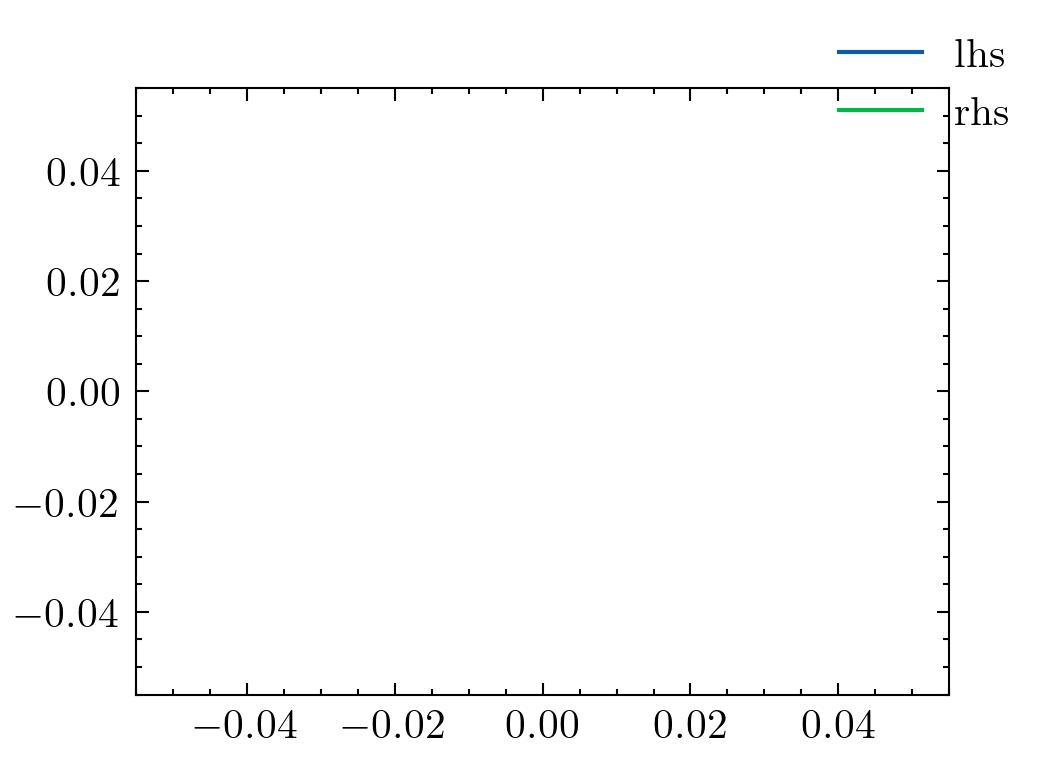
\includegraphics[width=0.7\linewidth]{media/fibergraphical}
%\end{figure}

\subsection{Modos HE y EH}
Interpretando (\ref{eqn:fiber_trascendental}) como una ecuación cuadrática en $J_\ell'(\alpha a)/\alpha a J_\ell(\alpha a)$:
\begin{align*}
	\frac{J_\ell'(\alpha a)}{\alpha a J_\ell(\alpha a)} &= -\left(\frac{n_1^2+n_0^2}{2n_1^2}\right) \frac{K_\ell'(\beta a)}{\beta a K_\ell(\beta a)}\pm\sqrt{\left(\frac{n_1^2-n_0^2}{2n_1^2}\right)^2\left(\frac{K_\ell'(\beta a)}{\beta a K_\ell(\beta a)}\right)^2+ \left( \frac{ k_z \ell}{ k_0 n_1} \right)^2\left[ \left(\frac{1}{\alpha a}\right)^2 + \left(\frac{1}{\beta a}\right)^2 \right]^2 }
\end{align*}

Si se hace uso de las relaciones de recurrencia de las funciones de Bessel $J_\ell(r)$,  es posible obtener dos tipos de soluciones que suelen ser llamadas HE y EH debido al campo longitudinal con mayor peso:
\begin{align}
		\frac{J_{\ell-1}(\alpha a)}{\alpha a J_\ell(\alpha a)} &= -\left(\frac{n_1^2+n_0^2}{2n_1^2}\right) \frac{K_\ell'(\beta a)}{\beta a K_\ell(\beta a)}+\frac{\ell}{(\alpha a)^2}-\sqrt{\Delta} \ , \quad \text{(modos HE)}
		\label{eqn:HE}
	\\
		\frac{J_{\ell+1}(\alpha a)}{\alpha a J_\ell(\alpha a)} &= \left(\frac{n_1^2+n_0^2}{2n_1^2}\right) \frac{K_\ell'(\beta a)}{\beta a K_\ell(\beta a)}+\frac{\ell}{(\alpha a)^2}-\sqrt{\Delta} \ , \quad \text{(modos EH)}
		\label{eqn:EH}
		\\
		\Delta &= \left(\frac{n_1^2-n_0^2}{2n_1^2}\right)^2\left(\frac{K_\ell'(\beta a)}{\beta a K_\ell(\beta a)}\right)^2+ \left( \frac{ k_z \ell}{ k_0 n_1} \right)^2\left[ \left(\frac{1}{\alpha a}\right)^2 + \left(\frac{1}{\beta a}\right)^2 \right]^2 \ . \nonumber
\end{align}
Para $\ell = 0$, se recuperan las relaciones obtenidas para los modos  TE$_m$ (HE$_{0m}$) y TM$_m$ (EH$_{0m}$). Para $\ell \neq 0$ se hace necesario considerar las expresiones asintóticas de las funciones de Bessel cuando $\beta a \to 0$ y $\alpha a \to V$:
\begin{align*}
	\frac{K'_\ell (x)}{xK_\ell (x)} &= -\frac{K_{\ell-1} (x)}{xK_\ell (x)}-\frac{\ell}{x^2}\approx \left\{\begin{matrix}
	\ln(xe^\gamma/2)-\frac{1}{x^2} \quad\text{si }\ell = 1
	\\
	-\frac{
	1}{2(\ell-1)}-\frac{\ell}{x^2}\quad \text{si }\ell > 1
	\end{matrix}\right. .
\end{align*}
El caso $\ell=1$ es de especial interés. La condición de modos HE se desarrolla como
\begin{align*}
	\frac{\alpha a J_1(\alpha a)}{J_0(\alpha a)} &= \left\{\left(\frac{n_1^2+n_0^2}{2n_1^2}\right) \left[ \ln\left(\frac{2}{e^\gamma \beta a}\right)+\frac{1}{(\beta a)^2} \right]+\frac{1}{(\alpha a)^2}-\sqrt{\Delta}\right\}^{-1} \to 0 \ .
\end{align*}
Basta considerar la función $J_1(\alpha a)|_{\alpha a \to V} = 0$. Por otro lado, la condición EH elimina el cero $x=0$ del cociente $\frac{\alpha aJ_1(\alpha a)}{J_2(\alpha a)}$ lo que hace que esté ``desfasada'' respecto a la condición HE. Usando un razonamiento similar al caso $\ell =0$, las condiciones de corte son
\begin{align*}
	(\lambda_c)_{1,m} &= 2\pi a \frac{\sqrt{n_1^2 - n_0^2}}{x_{1,m}} \ ,  \quad \left(\text{modos HE}_{1m}\right)
	\\
	(\lambda_c)_{1,m} &= 2\pi a \frac{\sqrt{n_1^2 - n_0^2}}{x_{1,m+1}} \ , \quad \left(\text{modos EH}_{1m}\right)
\end{align*}
con $x_{1,m}=$ 0, 3.832,  7.016, 10.173, $\dots$. En particular, el modo $\text{HE}_{11}$ siempre existe. Las longitudes de onda de corte finitas mayores son $\lambda_c \approx 252$ nm para los modos $\text{HE}_{12}$ y $\text{EH}_{11}$ 
El caso $\ell \ge 2$ tiene un desarrollo distinto por las forma asintóticas en juego y no será relevante para esta tesis. Sin embargo, se incluyen en la Figura \ref{fig:vortices} por completitud.
\begin{figure}[H]
	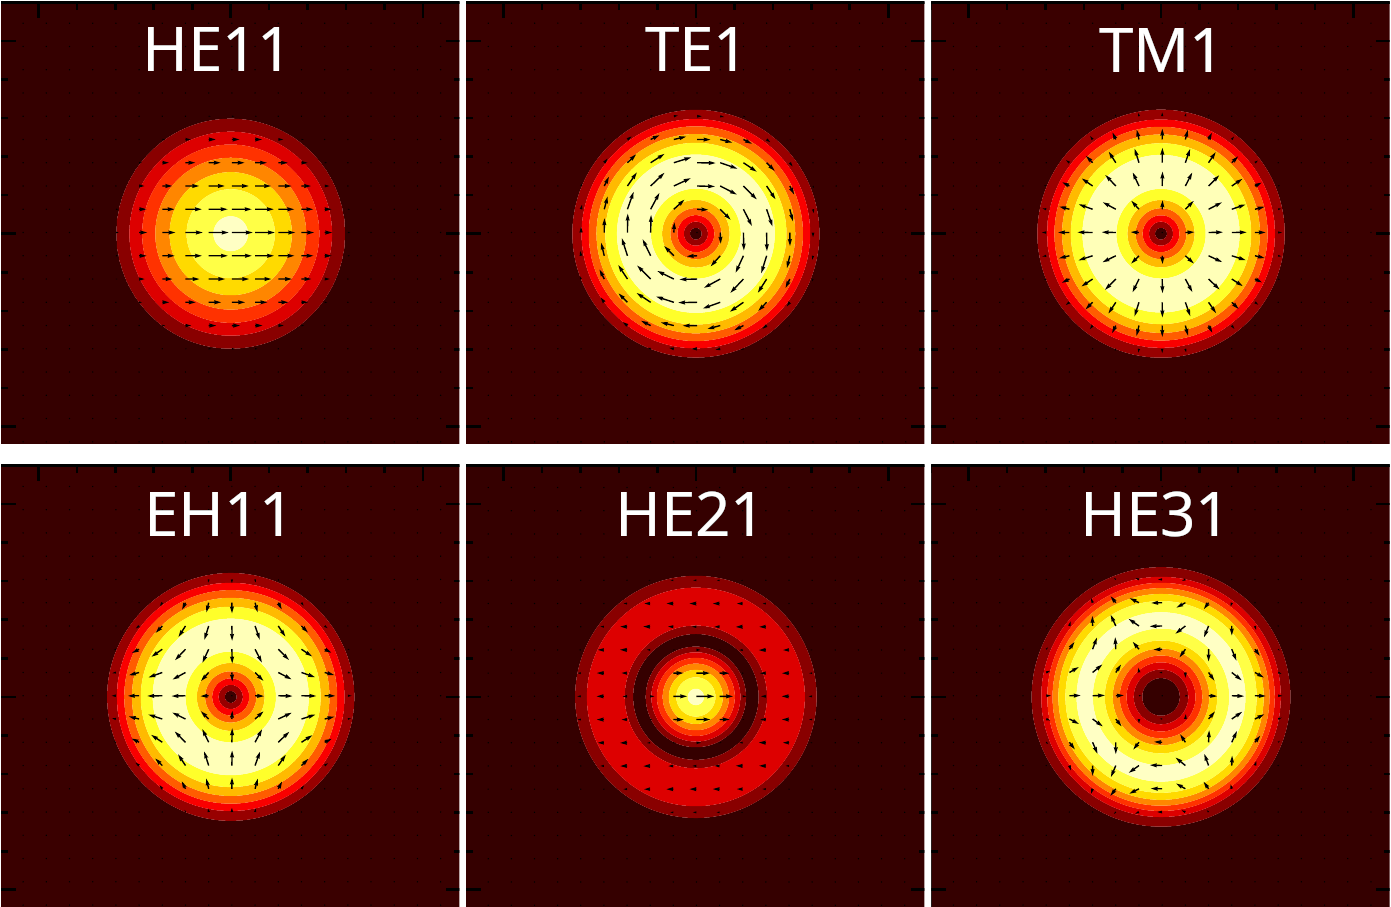
\includegraphics[width=\linewidth]{media/OAM_analitic}
		\caption{Primeros modos normales guiados para una guía circular o fibra óptica. \label{fig:vortices}}
\end{figure}

\section{Modos normales en guías de ondas}

Si la estructura de guías de ondas no varía en la dirección \( \hat{\textbf{z}} \), la solución para el campo eléctrico puede escribirse, por separación de variables, como una onda plana del tipo \( \textbf{E}(\textbf{r}) = \textbf{E}_\nu(x, y) e^{i\beta_\nu z} \). A su vez, resulta conveniente separar el operador laplaciano como \( \nabla^2 = \nabla_\perp^2 + \frac{\partial^2}{\partial z^2} \). 

Definiendo el operador \( D_{ij} \) tal que \( D_{ij} E_j \equiv \partial_i\left(\frac{\partial_j n^2}{n^2}E_j \right) \), la parte transversal de las ecuaciones de Helmholtz (\ref{eqn:helmholz}) puede escribirse como:
\begin{align}
	\begin{pmatrix}
		\nabla_\perp^2  + k_0^2n^2 + D_{xx} & D_{xy} 
		\\
		D_{yx}  & \nabla_\perp^2  + k_0^2n^2 + D_{yy} 
	\end{pmatrix}
	\begin{pmatrix}
		E_x
		\\
		E_y
	\end{pmatrix}
	=
	\beta_\nu^2 
	\begin{pmatrix}
		E_x
		\\
		E_y
	\end{pmatrix} \ . \label{eqn:eigenfield}
\end{align}

La ecuación (\ref{eqn:eigenfield}) constituye un problema de autovalores para \( \beta_\nu^2 \), cuyas autofunciones \( \textbf{E}_\nu^\perp(x,y) \) describen los perfiles transversales de los modos guiados. En general, se trata de un sistema vectorial acoplado de segundo orden, cuya resolución requiere técnicas numéricas. No obstante, en el régimen de \textit{guiaje débil}, en el que el índice de refracción varía levemente respecto a un fondo homogéneo \( n_0 \), se puede desacoplar el sistema y tratarlo como un problema escalar para una componente dominante del campo eléctrico\footnote{ver Apéndice \ref{sec:orto}.}.

Bajo esta aproximación, se suelen considerar modos cuasi-transversales, donde el campo eléctrico está principalmente polarizado en una dirección fija (por ejemplo, \( E_y \)), y la ecuación de Helmholtz se reduce a:
\begin{equation}
	\left[\nabla_\perp^2 + k_0^2 n^2(x,y) \right] \phi_\nu(x,y) = \beta_\nu^2 \phi_\nu(x,y) \ ,
\end{equation}
donde \( \phi_\nu(x,y) \) representa el perfil transversal del campo. Esta aproximación resulta válida para muchas geometrías experimentales, especialmente cuando la luz está polarizada linealmente y las variaciones del índice no inducen acoplamiento entre polarizaciones ortogonales.

Los modos obtenidos de esta ecuación permiten calcular las constantes de propagación \( \beta_\nu \), los perfiles espaciales del campo \( \phi_\nu(x,y) \), y otras magnitudes relevantes como los factores de confinamiento o las velocidades de grupo. Además, estos modos sirven como base para métodos posteriores, como la Expansión en Modos Normales (EME) o la Teoría de Modos Acoplados (CMT), utilizadas para describir la dinámica en redes fotónicas.
\section{Teoría de Modos Acoplados \label{cap:CMTteo}}
\subsection{Derivación desde un principio variacional}

A partir de las ecuaciones (\ref{eqn:EfieldH}) y (\ref{eqn:HfieldE}), es posible expresar la constante de propagación $k_z$ en términos del vector de Poynting $\textbf{S} = \frac{1}{2} \text{Re}\{\textbf{E} \times \textbf{H}^*\}$, siguiendo un desarrollo análogo al presentado en \citep{haus_coupled-mode}. 
\begin{equation}
	k_z = \frac{
		\frac{1}{4i} \iint \left[
		\left(-\nabla_\perp \times \textbf{E} + i\omega \mu_0 \textbf{H}\right) \cdot \textbf{H}^* 
		+ \left(\nabla_\perp \times \textbf{H} + i\omega \varepsilon_0 n^2 \textbf{E}\right) \cdot \textbf{E}^*
		\right] dxdy
	}{
		\frac{1}{4} \iint \left( 
		\textbf{E} \times \textbf{H}^* + \textbf{E}^* \times \textbf{H}
		\right) \cdot \hat{\textbf{z}} \, dxdy
	} \ . 
	\label{eqn:kzprevar}
\end{equation}
Al proponer una solución en forma de superposición de modos de las guías individuales del estilo
\begin{align*}
	\textbf{E} &= \sum_i a_i \textbf{e}_i \ , \quad \textbf{H} = \sum_i a_i \textbf{h}_i \ ,
\end{align*}
donde $a_i$ representa la amplitud del $i$-ésimo modo, los coeficientes permanecen indeterminados pero sujetos a minimizar la expresión para $k_z$. Sustituyendo estas expansiones en (\ref{eqn:kzprevar}), se obtiene una expresión simplificada para la constante de propagación del sistema $k_z$:
\begin{align*}
	(\textbf{E}\times\textbf{H}^* + \textbf{E}^*\times\textbf{H})\cdot\hat{\textbf{z}} 
	&= \sum_{ij} a_i^* \left( \textbf{e}_j \times \textbf{h}_i^* + \textbf{e}_i^* \times \textbf{h}_j \right) \cdot \hat{\textbf{z}} \, a_j 
	\equiv \sum_{ij} a_i^* p_{ij} a_j \ .
\end{align*}
El integrando del numerador se desarrolla como:
\begin{align*}
	\text{integrando numerador} &= i\sum_{ij} \Big[ a_i^* k_z^j (\hat{\textbf{z}}\times\textbf{e}_j )\cdot\textbf{h}_i^* a_j  + a_j \left(\omega \varepsilon_0 (n^2-n_j^2) \textbf{e}_j - k_z^j \hat{\textbf{z}}\times\textbf{h}_j \right) \cdot \textbf{e}_i^* a_i^* \Big] \ , \\
	&= i\sum_{ij} a_i^* \left[ k_z^j p_{ij} + \omega \varepsilon_0(n^2-n_j^2) \textbf{e}_j \cdot \textbf{e}_i^* \right] a_j \ ,
\end{align*}
donde $k_z^j$ es la constante de propagación del $j$-ésimo modo aislado\footnote{en general, $k_z \neq k_z^j$.}. 

Definiendo las siguientes cantidades fundamentales:
\begin{align}
	P_{ij} &\equiv \frac{1}{4} \iint \left( \textbf{e}_j \times \textbf{h}_i^* + \textbf{e}_i^* \times \textbf{h}_j \right) \cdot \hat{\textbf{z}} \ , dxdy, \label{eqn:pij-ori} \\
	&= \frac{1}{4 \omega \mu_0} \iint \Big[ 
	(k_z^i + k_z^j) \left( \textbf{e}_i^* \cdot \textbf{e}_j - e_{z,i}^* e_{z,j} \right)  + i \left( \textbf{e}_i^* \cdot \nabla_\perp e_{z,j} + \textbf{e}_j \cdot \nabla_\perp e_{z,i}^* \right) \Big] dxdy \ , \label{eqn:pij-simpli} \\
	H_{ij} &\equiv P_{ij} k_z^j + \frac{\omega \varepsilon_0}{4} \iint (n^2-n_j^2) \textbf{e}_j \cdot \textbf{e}_i^* \, dxdy \ , \label{eqn:hij}
\end{align}
se puede escribir la expresión (\ref{eqn:kzprevar}) para la constante de propagación $k_z$ de manera compacta como un cociente de Rayleigh-Ritz:
\begin{equation}
	k_z = \frac{\sum_{ij} a_i^* H_{ij} a_j}{\sum_{ij} a_i^*P_{ij} a_j} \ .
\end{equation}
Diferenciando con respecto a $a_k^*$ para optimizar el valor de $k_z$ se tiene:
\begin{align}
	\frac{\partial k_z}{\partial a_k^*} &= \frac{\sum_{ij} H_{ij} a_j \delta_{ik}}{\sum_{ij} a_i^*P_{ij} a_j} - \frac{\left(\sum_{ij} a_i^* H_{ij} a_j\right) \left( 
	\sum_{ij} \delta_{ik} P_{ij} a_j \right) }{\left(\sum_{ij} a_i^*P_{ij} a_j\right)^2} = \frac{\sum_{j} \left(H_{jk}  - k_z P_{kj} \right) a_j}{\sum_{ij} a_i^* P_{ij}a_j} \overset{!}{=} 0 \ .
\end{align}
Recuperando $k_z \to -i\frac{\partial}{\partial z}$, se obtienen las ecuaciones de $N$ modos acoplados no ortogonales:
\begin{equation}
	-i \sum_{j} P_{kj} \frac{d a_j}{dz} ´= \sum_{j} H_{kj} a_j \ , \text{ con }k=1,2,\cdots,N \ . \label{eqn:non-ortho-CMT-eqs}
\end{equation}
Claramente, de la expresión (\ref{eqn:pij-ori}) para $P_{ij}$, se cumple hermiticidad. A primera vista, puede parecer que $H_{ij}$ no es hermítica, pero veamos que sí lo es. Para ello, basta considerar la resta $H_{ij} - H_{ji}^*$ y notar que se anula:
\begin{align*}
 H_{ij} - H_{ji}^* &= P_{ij} k_z^j - P_{ji}^* k_z^i  + \frac{\omega \varepsilon_0}{4} \iint(n_i^2-n_j^2) \textbf{e}_i^* \cdot \textbf{e}_j dxdy
\\
&= \frac{1}{4} \iint (k_z^j-k_z^i)( \textbf{e}_j \times  \textbf{h}_i^* + \textbf{e}_i^* \times  \textbf{h}_j  )\cdot\hat{\textbf{z}} + \omega\varepsilon_0 (n_i^2-n_j^2) \textbf{e}_j \cdot \textbf{e}_i^* dxdy
\\
&= \frac{1}{4} \iint \left( i\nabla_\perp \times \textbf{e}_j +\omega\mu_0 \textbf{h}_j \right) \cdot \textbf{h}_i^* - \left( i\nabla_\perp \times \textbf{h}_j  - \omega\varepsilon_0n_j^2 \textbf{e}_j \right) \cdot \textbf{e}_i^*dxdy
\\
&- \frac{1}{4} \iint \left( i\nabla_\perp \times \textbf{e}_i^* +\omega\mu_0 \textbf{h}_i^*\right) \cdot \textbf{h}_j + \left(i\nabla_\perp \times \textbf{h}_i^*  + \omega\varepsilon_0n_i^2 \textbf{e}_i^* \right) \cdot \textbf{e}_jdxdy
\\
&+\frac{\omega\varepsilon_0}{4}\iint  \left(n_i^2-n_j^2\right) \textbf{e}_j \cdot \textbf{e}_i^* dxdy
\\
&= \frac{i}{4} \iint \left(\nabla_\perp\times\textbf{e}_j\right) \cdot \textbf{h}_i^*  -\left(\nabla_\perp\times\textbf{h}_j\right) \cdot \textbf{e}_i^* + \left(\nabla_\perp\times\textbf{e}_i^*\right) \cdot \textbf{h}_j - \left(\nabla_\perp\times\textbf{h}_i^*\right) \cdot \textbf{e}_j dxdy
\\
&= \frac{i}{4} \iint \nabla_\perp\cdot\left(\textbf{e}_j \times \textbf{h}_i^* +\textbf{e}_i^* \times \textbf{h}_j\right) dxdy =
\frac{i}{4} \oint_C \left(\textbf{e}_j \times \textbf{h}_i^* +\textbf{e}_i^* \times \textbf{h}_j\right) \cdot \hat{\textbf{n}} ds
\\
&=
0 \ ,
	\end{align*}
donde se ha usado que los campos deben decaer a cero en el infinito. Las ecuaciones (\ref{eqn:non-ortho-CMT-eqs}) se pueden obtener a partir de un Principio de Mínima Acción luego de definir el Lagrangiano $L$ de tipo campo discreto de Schrödinger:
\begin{equation}
	L = -\sum_{ij}  a_i^*\left(i  P_{ij} \frac{d }{dz} + H_{ij}  \right)a_j \ .
\end{equation}
Los momentos generalizados de este Lagrangiano son $\Pi_k=\frac{\partial L}{\partial \dot{a_k}} = -i\sum_{j} a_j^* P_{jk}$, por lo que el Hamiltoniano $H$ asociado es:
\begin{equation}
H = \sum_{j} \Pi_j \dot{a_j} - L = \sum_{ij} -ia_i^* P_{ij} \dot{a_j} + a_i^*\left(i  P_{ij} \frac{d a_j}{dz} + H_{ij} a_j \right) = \sum_{ij} a_i^* H_{ij} a_j \ .
\end{equation}
Dado que el Lagrangiano no depende explícitamtente de $z$, el Hamiltoniano $H$ es una cantidad conservada. Al variar el Lagrangiano se tiene:
\begin{align*}
	\delta L &= \sum_{ij} \frac{\partial L}{\partial a_j} \delta a_{j} +  \frac{\partial L}{\partial {a}_{i}^*} \delta {a}_{i}^* + \ \frac{\partial L}{\partial \dot{a}_{j}} \delta \dot{a}_{j} + \frac{\partial L}{\partial \dot{{a}}_{i}^*} \delta \dot{{a}}_{i}^*
	\\
	&= \sum_{ij} \left( \frac{\partial L}{\partial a_{j}} - \frac{d}{dz}\frac{\partial L}{\partial \dot{a}_{j}} \right)\delta a_{j} + \left( \frac{\partial L}{\partial {a}_{i}^*} - \frac{d}{dz}\frac{\partial L}{\partial  \dot{{a}}_{i}^*} \right)\delta {a}_{i}^* + \frac{d}{dz}\left(\frac{\partial L}{\partial \dot{a}_{j}}\delta a_{j} +  \frac{\partial L}{\partial \dot{{a}}^*_{i}}\delta {a}_{i}^*\right)
	\\	
	&\implies  \frac{d}{dz} \sum_{ij}\left(\frac{\partial L}{\partial \dot{a}_{j}}\delta a_{j} +  \frac{\partial L}{\partial \dot{{a}}_{i}^*}\delta {a}_{i}^*\right) = 0 \ .
\end{align*}
El par de transformaciones asociadas al grupo unitario U(1), $a_j\to a'_j = e^{i\phi}a_j$, ${a}_i^* \to {a'}_i^* = e^{-i\phi}{a}_i^*$ dejan invariante el Lagrangiano, y si se toma una variación infinitesimal $\phi \ll 1$ se tiene $\delta a_j = i\phi a_j$ y $\delta {a}_i^* = -i\phi {a}_i^*$, por lo que la cantidad conservada, $P$, que se identifica con la potencia total del sistema y está directamente relacionada con el vector de Poynting es:
\begin{equation}
	P = \sum_{ij} a_i^* P_{ij} a_j = \iint \textbf{S} \cdot \hat{\textbf{z}} dxdy \ .  \label{eqn:power}
\end{equation}
Se tienen entonces dos cantidades conservadas en la dinámica, $H$ y $P$, que serán de utilidad para verificar la validez de soluciones numéricas a la ecuación (\ref{eqn:non-ortho-CMT-eqs}).

\subsection{Dímero TE en guías de ondas tipo placa}
Mediante las ecuaciones de las componentes transversales (\ref{eqn:transversal}) en el caso de modos TE fundamentales (\ref{eqn:TEanti}), se tiene: 
\begin{align*}
	\textbf{e}_{j\perp} &= \hat{\textbf{y}}\frac{i\omega\mu_0 H_{a1}}{k_0^2n_j^2 - (k_z^j)^2}\left\{ \begin{matrix}
-\alpha \cos(\alpha (x-x_j)), &|x-x_j|\le a
\\
\beta\sin(\alpha a) e^{-\beta(|x-x_j|-a)}, &|x-x_j| > a
\end{matrix}\right. \ ,
\\
\textbf{h}_{j\perp} &= \hat{\textbf{x}}\frac{ik_z^j H_{a1}}{k_0^2n_j^2 - (k_z^j)^2}\left\{ \begin{matrix}
\alpha \cos(\alpha (x-x_j)), &|x-x_j|\le a
\\
-\beta\sin(\alpha a) e^{-\beta(|x-x_j|-a)}, &|x-x_j| > a
\end{matrix}\right. \ ,
\end{align*} con $x_j=jd$, $d\ge 2a$ y $L=\int dy$. Elementos no diagonales tienen la forma:
\begin{align*}
	\left(\textbf{e}_{j\perp}\times\textbf{h}_{i\perp}^*\right)\cdot \hat{\textbf{z}}
	&=
	\frac{k_z^i \omega \mu_0 H_{a1}^2 \beta\sin(\alpha a)}{(k_0^2n_j^2 - k_z^2)(k_0^2n_i^2 - k_z^2)}
	\left\{
	\begin{matrix}
		 \alpha\cos(\alpha(x-x_i))e^{-\beta(|x-x_j|-a)}, & |x-x_i| \le a
		\\
		i \leftrightarrow j, & |x-x_j| \le a
		\\
		\beta \sin(\alpha a)e^{-\beta (|x-x_i|+|x-x_j|-2a)}, & \text{otro caso}
	\end{matrix}
	\right. \ ,
\\
	P_{ij} &= \frac{L k_z^i k_0  \mu_0 c H_{a1}^2 \sin^2(\alpha a)e^{-\beta d}e^{\beta a}}{2\beta} \left[\frac{e^{-\beta a} + \beta (d-2a)e^{\beta a}}{\beta^2} - \frac{2\cosh(\beta a)}{\alpha^2+\beta^2} \right] \ ,
\\
	\tilde{H}_{ij} &\equiv H_{ij} - P_{ij} k_z^j = \frac{L k_0    \mu_0 c H_{a1}^2 }{2 \beta }  \sin^2(\alpha a)e^{2\beta a} e^{-\beta d} \ .
\end{align*}
Elementos diagonales tienen la forma:
\begin{align*}
	\left(\textbf{e}_{j\perp}\times\textbf{h}_{j\perp}^*\right)\cdot \hat{\textbf{z}}&=\frac{k_z^j\omega\mu_0 H_{a1}^2}{(k_0^2n_j^2-k_z^2)^2} \left\{ \begin{matrix}
\alpha^2\cos^2(\alpha (x-x_j)), & |x-x_j| \le a
\\
\beta^2 \sin^2(\alpha a) e^{2\beta a} e^{-2\beta|x-x_j|}, & |x-x_j|>a
\end{matrix}\right. \ ,
\\
	P_{jj} &= \frac{L k_z^j  k_0 \mu_0 c H_{a1}^2  a}{2 \alpha^2} \left[1 + \frac{\sin^2(\alpha a)}{a \beta^3 } k_0^2 \left( n_1^2 - n_0^2 \right) \right] \ ,
\\
	\tilde{H}_{jj} &\equiv H_{jj} - P_{jj} k_z^j =
	\frac{L k_0^3  \mu_0 c H_{a1}^2 \sin^2(\alpha a)e^{2\beta a}e^{-2\beta d}}{4 \beta^3 } (n_1^2-n_0^2) \sinh(2\beta a) \ .
\end{align*}
La dinámica está regida por el sistema acoplado de las ecuaciones (\ref{eqn:non-ortho-CMT-eqs}), que luego de premultiplicar por la inversa de la matriz $P_{ij}$ toma la forma compacta:
\begin{align*}
	-i\frac{d}{dz}\begin{pmatrix}
	a_1
	\\
	a_2
	\end{pmatrix} &= 	
	\begin{pmatrix}
	\tilde{k} & C
	\\
	C & \tilde{k}
	\end{pmatrix}
	\begin{pmatrix}
	a_1
	\\
	a_2
	\end{pmatrix} \ ,
\end{align*}
con, por ejemplo, $\tilde{k}\equiv k_z^{\text{TE}} + \delta k$, $k_z^{\text{TE}} \sim 1.3\times10^5 \text{ cm}^{-1}$, $C\equiv \frac{P_{ii} \tilde{H}_{ij}  -P_{ij}\tilde{H}_{ii}}{P_{ii}^2-P_{ij}^2} \sim 1\text{ cm}^{-1}$ y $\delta k \equiv \frac{P_{ii} \tilde{H}_{ii} -P_{ij}\tilde{H}_{ij}}{P_{ii}^2-P_{ij}^2} \sim -0.02\text{ cm}^{-1}$ para $\lambda = 730$ nm, $n_1 = n_0 + 4\times10^{-4}$ y una distancia entre guías de $d = 18 $ $\mu$m. La matriz $\hat{P}^{-1}\hat{H}$ se puede escribir en términos de las matrices de Pauli como $\tilde{k}I + C\sigma_x $, lo que permite utilizar sus propiedades para resolver la dinámica del sistema:
\begin{align*}
	\begin{pmatrix}
	a_1(z)
	\\
	a_2(z)
	\end{pmatrix}
	=
	e^{{i\left[\tilde{k}I + C\sigma_x\right]z }}	\begin{pmatrix}
	a_1(0)
	\\
	a_2(0)
	\end{pmatrix}
	=
	e^{i\tilde{k}z}
	\begin{pmatrix}
	\cos(Cz) & i\sin(Cz)
	\\
	i\sin(Cz) & \cos(Cz)
	\end{pmatrix}
	\begin{pmatrix}
	a_1(0)
	\\
	a_2(0)
	\end{pmatrix} \ .
\end{align*}
Una forma de encontrar el valor experimental del acoplamiento $C$ es mediante la excitación individual de un modo. Con esto, la razón entre las potencias $|a_1(z)|^2$ y $|a_2(z)|^2$ permite despejar el acoplamiento para una distancia de propagación $z=L<\frac{\pi}{2C}$ conocida:
\begin{equation}
	C = \frac{1}{L}\tan^{-1}\left( \left|\frac{a_2(L)}{a_1(L)}\right|^2 \right) \ . \label{eqn:coupling-simp}
\end{equation}
\subsection{Bandas y Topología: Red de Su-Schrieffer-Heeger fotónica}
Si bien es posible reformular las ecuaciones de Maxwell como un problema de autovalores en simulitud con la mecánica cuántica para plantear un análogo al teorema de Bloch \cite{joannopoulos_photonic_2008}, la matriz $\hat{C}\equiv\hat{P}^{-1}\hat{H}$ hermítica de la ecuación (\ref{eqn:non-ortho-CMT-eqs}) es justificación suficiente para invocarlo: Es posible expresar las soluciones del sistema en una base de cuasimomento cuya periodicidad sea la misma que la de la matriz $\hat{C}$.
Para ejemplificar lo anterior se usará el célebre modelo de Su-Schrieffer-Heeger (SSH), que es uno de los sistemas más sencillos que exhibe \textit{estados de borde topológicos} \cite{ssh, ssh-photonic, topological-photonics}. Originado para explicar la formación de estados electrónicos localizados en el poliacetileno, consiste en considerar únicamente dos tipos de acoplamiento: uno fuerte (enlace doble) y uno débil (enlace simple). En términos de Física del Estado Sólido, corresponde a una red unidimensional con base de dos sitios, cuyas amplitudes modales se denotan $a_n$ y $b_n$. En la Figura \ref{fig:ssh-model} se ilustra el modelo a estudiar, que se corresponde al siguiente Hamiltoniano $H$. 
\begin{equation*}
	H = \sum_n \left( t b_n^*a_n + t'  a_{n+1}^*b_n  + c.c. \right) \ .
\end{equation*}
\begin{figure}[h]
\centering
	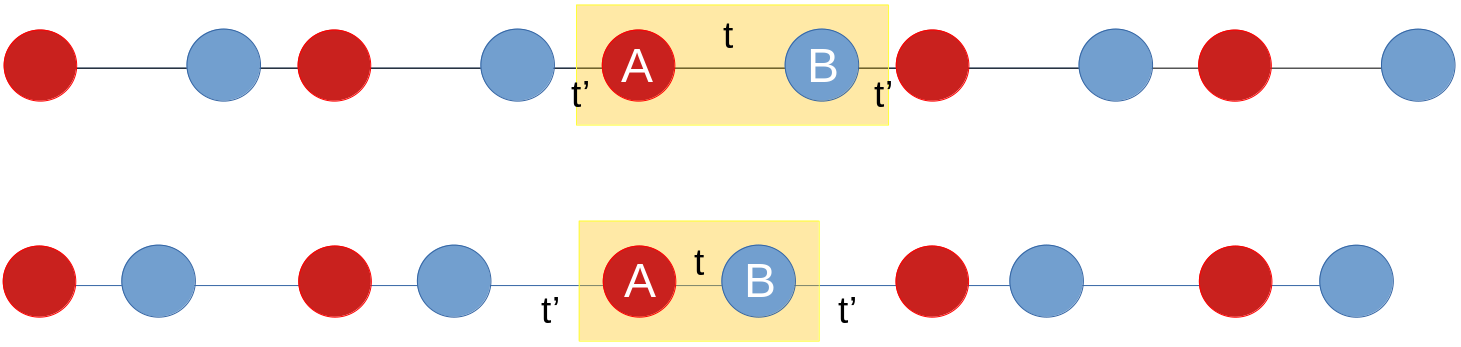
\includegraphics[width=\linewidth]{media/ssh-model.png}
	\caption[Esquema del modelo SSH.]{Esquema del modelo SSH. En amarillo se encierra la celda unitaria, donde se distinguen los sitios A y B y el acoplamiento intracelda (intercelda) $t$ ($t'$). Se muestran dos configuraciones distintas. \label{fig:ssh-model}}
\end{figure}
En condiciones de borde periódicas (Born-von Karman), es posible diagonalizar el Hamiltoniano en la base de Bloch con $a_n = \frac{1}{\sqrt{N}}\sum_k a_k e^{iknd}$, $b_n = \frac{1}{\sqrt{N}}\sum_k b_k e^{iknd}$ de la siguiente forma:
\begin{align*}
	H &= \frac{1}{N}\sum_n \sum_{k k'} \left[\left(t + t' e^{ikd}\right) a_k b_{k'}^* e^{i(k-k')nd}  + \left(t  + t' e^{-ikd}\right) a_k^* b_{k'} e^{-i(k-k')nd} \right]
	\\
	&=  \sum_k 
	\begin{pmatrix}
		a_k^* & b_k^*		
	\end{pmatrix}
	\underbrace{
	\begin{pmatrix}
		0 & t+ t'e^{-ikd}
		\\
		t+ t'e^{ikd} & 0
	\end{pmatrix}}_{\hat{H}(k)}
	\begin{pmatrix}
		a_k
		\\
		b_k		
	\end{pmatrix},
\end{align*}
donde se ha usado que $$\frac{1}{N}\sum_n e^{i(k-k')nd} = \left\{\begin{matrix} \frac{N}{N}=1, &\text{ si } k = k'
\\ \frac{1}{N}\frac{1-\cancelto{1}{e^{i(k-k')Nd}}}{1-e^{i(k-k')d}}e^{i(k-k')d}=0, &\text{ si } k\neq k'
\end{matrix}\right. =\delta_{kk'},$$ pues $k, k' \in  \left\{\frac{2\pi l}{Nd}, l=0,\pm 1, \dots , \pm \frac{N}{2}\right\}$ pertenecen a la red recíproca 1D. El espectro de $\hat{H}(k)$ es $\lambda_k = \pm\sqrt{t^2+t'^2+2tt'\cos(kd)}$, lo que pareciera indicar que el sistema es simétrico entre $t$ y $t'$. Sin embargo, el cuadro no está completo sin los autovectores de $\hat{H}(k)$, $\textbf{v}_\pm =\frac{1}{\sqrt{2}} \begin{pmatrix} \pm e^{-i\phi(k)} \\  1 \end{pmatrix}$, con $\phi(k)=\tan^{-1}\left(\frac{t'\sin(kd)}{t+t'\cos(kd)}\right)$. Si se define el vector $\textbf{d}(k) \equiv \begin{pmatrix}t+t'\cos(kd) \\ t'\sin(kd) \\ 0 \end{pmatrix}$ es posible escribir el Hamiltoniano $\hat{H}(k)$ en términos de las matrices de Pauli $\hat{H}(k) = \textbf{d} \cdot \bm{\sigma} = d_x\sigma_x + d_y\sigma_y$. Este vector $\textbf{d}(k)$ es una representación vectorial del Hamiltoniano de bulto de 2$\times$2 en el espacio de momentum. La fase $\phi(k)$ se relaciona con el ángulo que forma la proyección del vector $\textbf{d}(k)$ en el plano $xy$,  $\phi(k)=\tan^{-1}\left( \frac{d_y}{d_x} \right)$. En particular, cuando $\delta \equiv t/t' < 1$, el vector $\textbf{d}(k)$ encierra el origen una vez, mientras que para $\delta > 1$ no se encierra el origen, como se aprecia en la Figura \ref{fig:ssh-topo}. Formalmente, las fases de Zak, $\mathcal{Z}_\pm$, asociadas a los autoestados del bulto (zona lo suficientemente alejada de los bordes) cambian dependiendo del valor de $\delta$. Por definición \citep{zak_berry}, \begin{align*}
\mathcal{Z}_\pm &= i \oint \textbf{v}_\pm^\dagger \frac{d \textbf{v}_\pm}{dk}  dk  = -\frac{1}{2} \int_{-\frac{\pi}{d}}^{{\frac{\pi}{d}}}  \frac{d \phi(k)}{d k} dk = -\frac{d}{2}\int_{-\frac{\pi}{d}}^{{\frac{\pi}{d}}} \frac{1+\delta\cos(kd)}{\delta^2+1+2\delta\cos(kd)} dk = -\frac{\pi}{2} \left(1 + \frac{1-\delta^2}{\left|1-\delta^2\right|} \right) \ .
\end{align*}
Es decir, 
\begin{align*}
\mathcal{Z}_\pm &= \left\{\begin{matrix}
-\pi, &\text{ si } |\delta| < 1
\\
0, &\text{ si } |\delta| > 1
\end{matrix}\right. \ .
\end{align*}
El cambio en la fase de Zak al variar el parámetro $\delta$  se conoce como \textit{transición topológica} puesto que no es posible pasar de un régimen a otro de forma suave. Esto tiene implicancias en el sistema con condiciones de borde abiertas (Dirichlet) debido a la \textit{correspondencia bulto-borde} \cite{topobulk}. En concreto, así como se ilustra en la Figura \ref{fig:ssh-open}, la topología del Hamiltoniano $\hat{H}(k)$ induce la aparición de estados de borde a energía cero al imponer condiciones de borde abiertas.
El Hamiltoniano del modelo SSH presenta diversas simetrías: de reversión temporal, de inversión, partícula-hueco, traslacional y quiral. Esta última es de particular relevancia, pues los estados de borde del modelo SSH están \textit{topológicamente protegidos} ante cualquier desorden que respete la simetría quiral \cite{ssh-course}. El operador quiral en cuestión es la matriz de Pauli $\sigma_z$, pues 
\begin{align*}
	\left\{\hat{H}(k), \sigma_z \right\} = \left\{d_x \sigma_x + d_y\sigma_y , \sigma_z \right\} = d_x \cancelto{0}{\left\{\sigma_x, \sigma_z \right\}} + d_y \cancelto{0}{\{\sigma_y, \sigma_z\}} = 0 \ .
\end{align*}
\begin{figure}[h]
	\centering
	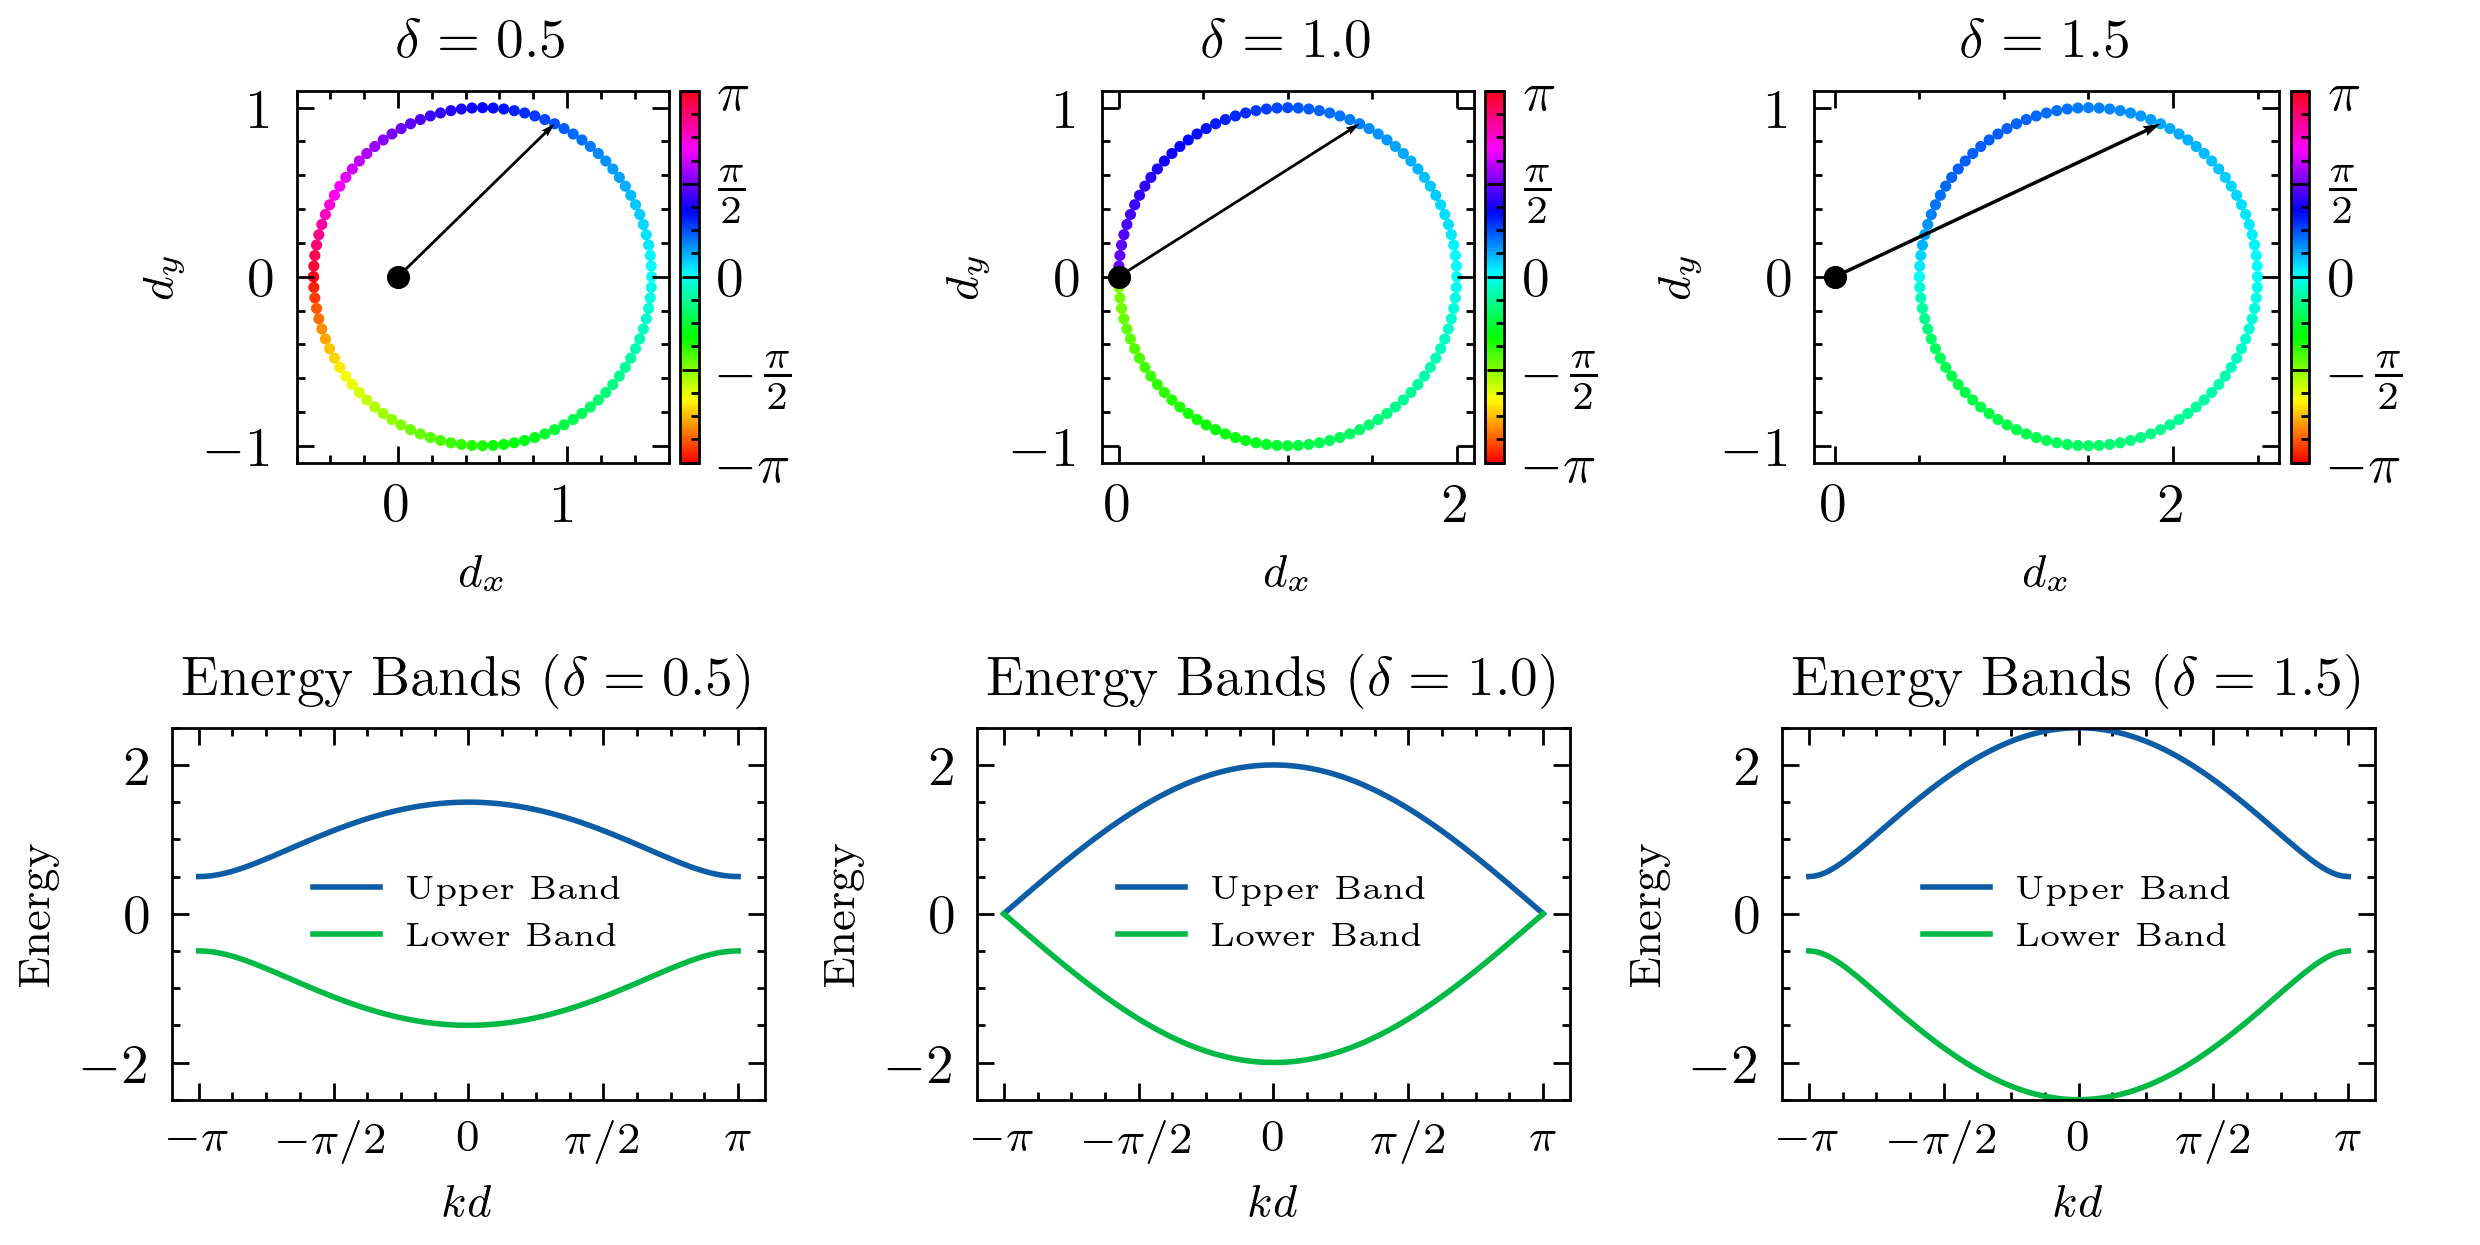
\includegraphics[width=\linewidth]{media/ssh-winding}
	\caption[Topología de la red SSH.]{Topología de la red SSH. Arriba: Vectores $\textbf{d}$(k) y su fase. Para $\delta < 1$ ($\delta > 1$), (no) se encierra el origen. Abajo: Bandas en función del cuasimomento $k$ en la primera zona de Brillouin para $\delta < 1$, $\delta = 1$ y $\delta > 1$. Se fija $t'=1$ y se varía $\delta'$ para un número $N=100$ de celdas unitarias. 
	\label{fig:ssh-topo}}
\end{figure} \begin{figure}[h]
\centering	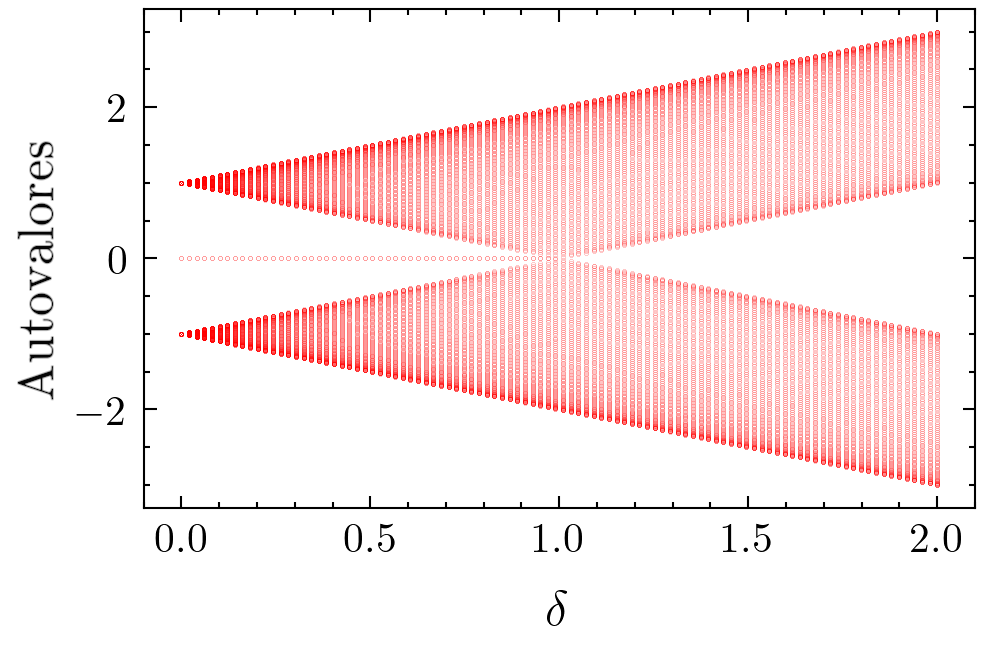
\includegraphics[width=0.7\linewidth]{media/ssh-open}
	\caption[Espectro de la red SSH.]{Espectro de la red SSH finita. Se aprecia la aparición de los estados de borde a energía cero para $\delta < 1$. Condiciones de borde abiertas en función del parámetro $\delta=t/t'$, para $t'=1$ fijo y para un número $N=100$ de celdas unitarias.
	\label{fig:ssh-open}}
\end{figure} 
